\documentclass[tikz, border=1cm]{standalone}

\definecolor{ACMOrange}{RGB}{252, 146, 0}
\definecolor{ACMRed}{RGB}{253, 27, 20}
\definecolor{ACMPurple}{RGB}{101, 1, 107}

\begin{document}

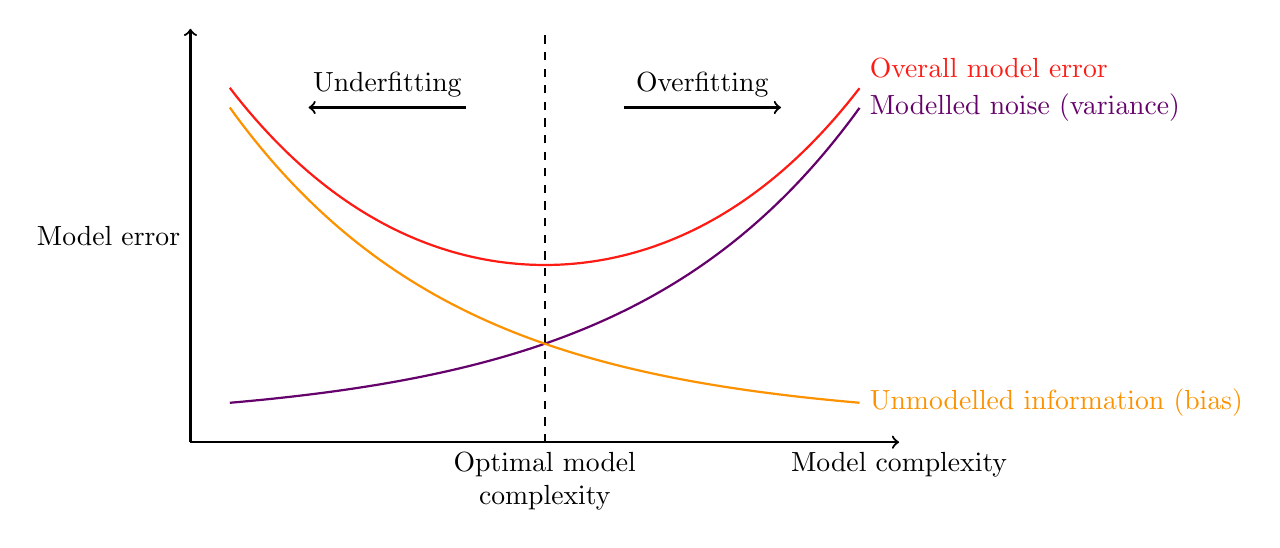
\begin{tikzpicture}[scale=2, domain=-2:2, y=0.5cm]

\draw[->, thick] (-2.25,-0.25) -- (2.25,-0.25) node [below] {Model complexity};
\draw[->, thick] (-2.25,-0.25) -- (-2.25,5) node [midway, left] {Model error};

\draw[dashed, thick] (0,-0.25) node [below, text width=3cm, align=center] {Optimal model complexity} -- (0,5) ;

\draw[->, thick] (-0.5,4) -- (-1.5,4) node [midway, above] {Underfitting};
\draw[->, thick] (0.5,4) -- (1.5,4)node [midway, above] {Overfitting};

\coordinate (O) at (0,0);

\draw[ACMRed, thick] plot[samples=100] (\x, {2^\x + 2^(-\x)}) node[above right] {Overall model error};
\draw[ACMPurple, thick] plot[samples=100] (\x, {2^(\x)}) node[right] {Modelled noise (variance)};
\draw[ACMOrange, thick] plot[samples=100] (\x, {2^(-\x)}) node[right] {Unmodelled information (bias)};

\end{tikzpicture}
\end{document}